\documentclass[conference]{IEEEtran}
\IEEEoverridecommandlockouts
% The preceding line is only needed to identify funding in the first footnote. If that is unneeded, please comment it out.
\usepackage{cite}
\usepackage{amsmath,amssymb,amsfonts}
\usepackage{algorithmic}
\usepackage{graphicx}
\usepackage{textcomp}
\usepackage{xcolor}
\usepackage[english, brazil]{babel}
\def\BibTeX{{\rm B\kern-.05em{\sc i\kern-.025em b}\kern-.08em
    T\kern-.1667em\lower.7ex\hbox{E}\kern-.125emX}}
\begin{document}

\title{Análise da influência da renda familiar na evasão de alunos no Instituto Federal de Educação, Ciência e Tecnologia de São Paulo}

\author{\IEEEauthorblockN{Luiz Roberto Albano Junior}
\IEEEauthorblockA{\textit{Faculdade de Engenharia Elétrica e de Computação} \\
\textit{Universidade Estadual de Campinas}\\
Campinas, Brasil \\
l272746@g.unicamp.br}
\and
\IEEEauthorblockN{Tárcio Augusto Canhamina Quissanga}
\IEEEauthorblockA{\textit{Faculdade de Engenharia Elétrica e de Computação} \\
\textit{Universidade Estadual de Campinas}\\
Campinas, Brasil \\
t214551@dac.unicamp.br}
}

\maketitle

\selectlanguage{brazil}
\begin{abstract}
    Este estudo investiga a influência da renda familiar na evasão de alunos no Instituto Federal de Educação, Ciência e Tecnologia de São Paulo (IFSP). A evasão escolar, definida como a saída definitiva do estudante do seu curso sem conclusão, representa um desafio significativo para as instituições de ensino, impactando tanto o funcionamento institucional quanto o aproveitamento dos recursos públicos. Utilizando microdados das matrículas disponíveis na Plataforma Nilo Peçanha (PNP), este trabalho busca avaliar se a evasão dos estudantes é influenciada pela renda familiar. Foram aplicadas técnicas de análise estatística e visualização de dados, com a hipótese nula (H0) postulando que a evasão não é influenciada pela renda familiar. Os resultados são analisados através da distribuição qui-quadrado para verificar a independência das variáveis e técnicas de reamostragem para determinar intervalos de confiança. A pesquisa também identifica outras possíveis variáveis que possam influenciar a evasão escolar, oferecendo uma compreensão abrangente do fenômeno e contribuindo para estratégias de retenção mais eficazes no IFSP.\\
\textbf{Palavras chave: } evasão escolar, análise estatística, teste de hipótese, microdados educacionais
\vspace{2.5mm}
\end{abstract}

\selectlanguage{english}
\begin{abstract}
    This study investigates the influence of family income on student dropout rates at the Federal Institute of Education, Science and Technology of São Paulo (IFSP). School dropout, defined as the permanent exit of a student from a course without completing it, represents a significant challenge for educational institutions, impacting both institutional functioning and the use of public resources. Using microdata from enrollments available on the Nilo Peçanha Platform (PNP), this work seeks to assess whether student dropout rates are influenced by family income. Statistical analysis and data visualization techniques were applied, with the null hypothesis (H0) postulating that dropout rates are not influenced by family income. The results are analyzed using the chi-square distribution to verify the independence of the variables and resampling techniques to determine confidence intervals. The research also identifies other possible variables that may influence school dropout rates, offering a comprehensive understanding of the phenomenon and contributing to more effective retention strategies at IFSP.\\
\textbf{Keywords: } school dropout, statistical analysis, hypothesis testing, educational microdata
\end{abstract}

\section{Introdução}
Um dos maiores desafios enfrentados pelas instituições de ensino é o problema da evasão de estudantes. Este problema complexo que pode se originar de diversos fatores e que impacta diretamente tanto estudantes quanto o funcionamento das instituições educacionais \cite{oliveira2021}.\par
Podemos definir a evasão como a saída definitiva do estudante de seu curso de origem, sem concluí-lo. As formas de evasão podem ocorrer de diversas maneiras, como o abandono dos estudantes às aulas, exauridas as tentativas de contato, pela desistência formalizada pelo estudante, a transferência para outra instituição ou a exclusão por ação institucional \cite{silveira2021}.\par
No contexto do Instituto Federal de Educação, Ciência e Tecnologia de São Paulo (IFSP), a evasão compromete o funcionamento e a eficiência da instituição, causando impacto financeiro significativo. Este impacto é causado pela perda de receitas, enquanto os custos operacionais permanecem inalterados, podendo resultar na ociosidade de professores, funcionários, equipamentos e espaços físicos, representando um desperdício de recursos públicos ou a depreciação destes serviços \cite{silveira2021}.\par
Diversos fatores contribuem para a evasão escolar. De forma externa, analisando o lado do estudante, podemos destacar fatores como formação educacional deficitária, falta de identificação com o curso escolhido e problemas socioeconômicos, objetivo de análise deste artigo, como a baixa renda familiar ou a necessidade de conciliar trabalho e estudo. Além disso, problemas internos como disciplinas com alto grau de dificuldades, falta de preparo pedagógico de docentes e a carga horária de alguns cursos agravam a situação dos estudantes.\par
Compreender a evasão escolar no IFSP, e em outras instituições de ensino, exige uma atenção e esforços contínuos para identificação dos fatores e variáveis que contribuem com o problema, além de esforços coordenados para redução do problema, mantendo os alunos na instituição e possivelmente assegurando que eles tenham uma experiência educacional mais significativa e de qualidade.\par
O propósito deste trabalho é avaliar a partir de dados abertos disponíveis na plataforma Plataforma Nilo Peçanha (PNP) \cite{pnp2024}, se a evasão dos estudantes desta instituição são influenciadas pela renda familiar. Serão utilizadas ferramentas como gráficos e de conceitos de análise estatística, de hipóteses e estatísticas de teste que possam confirmar a afirmação inicial, ou hipótese nula ("H-nada") \cite{ismay2024}, de que a evasão dos alunos do Instituto Federal de São Paulo (IFSP) não é influenciada pela renda familiar. Além disso, tentar identificar outras possíveis variáveis da base de dados poderiam causar influência na evasão escolar.


\section{Materiais e Métodos}
Para realização deste estudo utilizamos os microdados referentes às matrículas dos estudantes, contidos no Portal de Dados Abertos do Ministério da Educação - Plataforma Nilo Peçanha (PNP) \cite{pnpdados2024}. A base de dados escolhida {microdados2021} foi a mais recente disponível no momento do acesso, representando um conjunto de dados de matrículas de estudantes que estiveram pelo menos um dia do ano base de 2020.\par
A documentação foi realizada em um \textit{notebook Python} disponível em \cite{notebook}. Para elaboração do \textit{notebook} foi utilizada a linguagem de programação Python \cite{python2024} e bibliotecas para manipulação, análise de dados, computação de modelos estatísticos e análise visual de dados, sendo: Pandas \cite{pandas2024}, NumPy \cite{numpy2024}, Plotnine \cite{plotnine20204}, Matplotlib \cite{matplot2024}, Seaborn \cite{seaborn2024}, SciPy \cite{scipy2024} e Statsmodel \cite{statsmodel2024}.\par
O primeiro passo foi realizar uma visualização bruta de alguns dados para visualização de categorias de valores e realização da limpeza de dados inexistentes que pudessem comprometer as futuras análise e exploração das variáveis.\par
Como a base de dados contém informações de matrículas de toda rede federal de ensino, foi-se necessário a aplicação de um filtro na coluna "Instituição" para o valor "IFSP", a fim de aproximar do objetivo desta análise.\par
A análise inicial realizada foi verificar os valores contidos na variável "Situação de Matrícula", que continham os dados necessários para a definição de uma matrícula que caracteriza-se pela evasão de um estudante. A Figura 1 nos permite ver as categorias de valores e seus totalizadores.\par

\begin{figure}[h]
    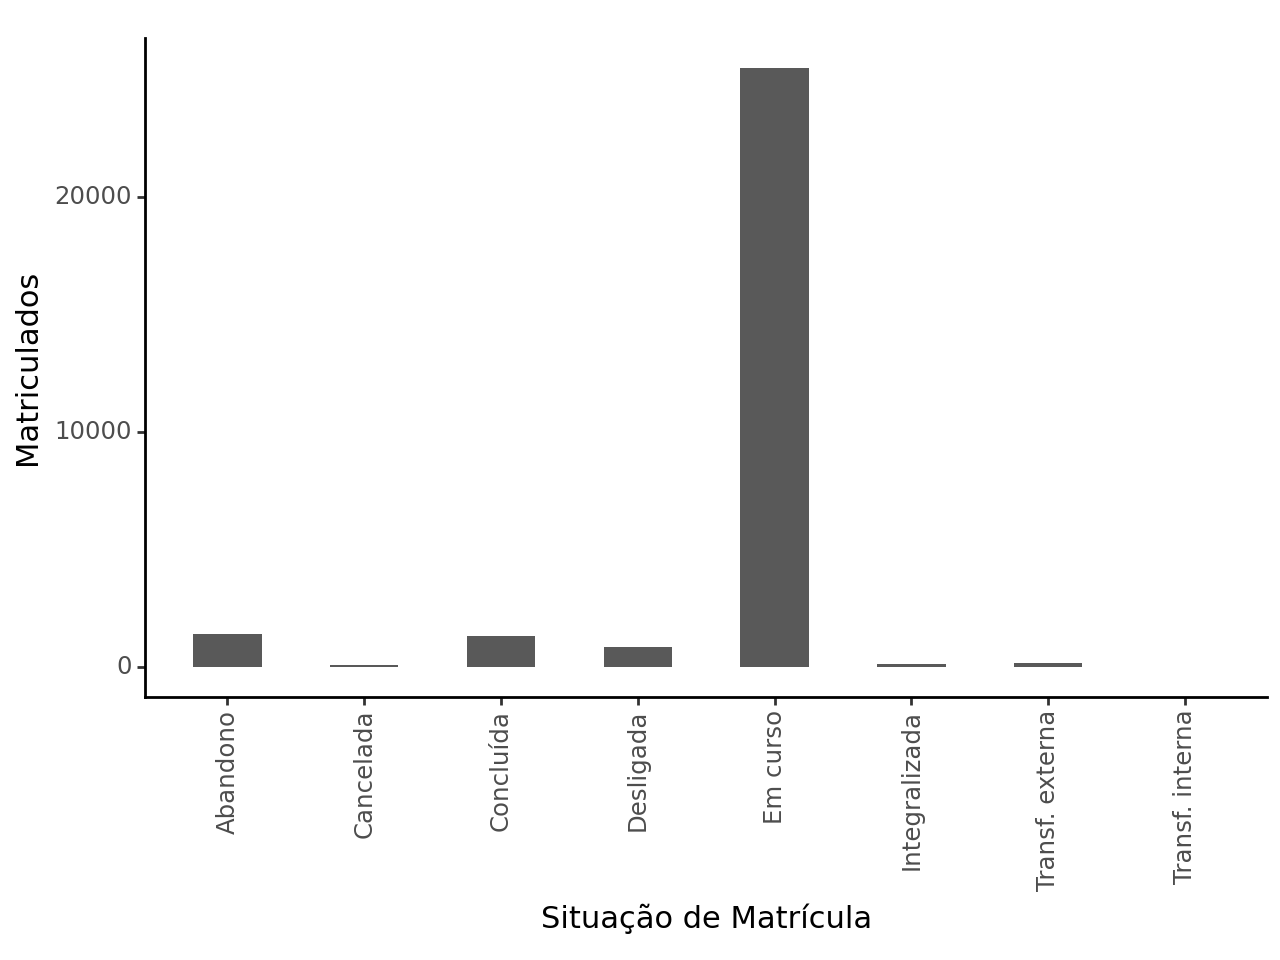
\includegraphics[width=8.9cm]{figs/figura-1.png}
    \centering
    Figura 1. Gráfico do tipo histograma representando o total de registros de matrículas por situação.
\end{figure}

A visualização destes dados permitiu a definição de quais situações de matrículas representavam a evasão de um estudante. Seguindo a caracterização de evasão definida pela Comissão de Especial de Estudos sobre a Evasão nas Universidades Públicas Brasileiras, criada em 1995, durante o Seminário sobre Evasão nas Universidades Brasileiras \cite{silveira2021}, caracterizam-se como evasão as seguintes situações de matrículas: "Abandono", "Cancelada", "Desligada" e "Transferência Externa". Com esta caracterização uma nova variável foi adicionada à base de dados, classificando os registros como "Evadidos" e "Não Evadidos".\par
A partir desta análise dos totais de matrículas houve a necessidade de refinar ainda mais a base de dados, eliminando o número de matrículas cuja renda familiar não foi informada e também filtrando as matrículas pelos cursos da formação básica brasileira, de acordo com a Lei de Diretrizes e Bases da Educação Nacional, que no âmbito dos cursos oferecidos pelo IFSP abrangem o ensino médio e técnico, e também os cursos de formação inicial do nível superior.\par
Na sequência através da exploração e análise dos dados, utilizando-se de histogramas foram visualizadas o comportamento das principais variáveis presentes na base de dados escolhida, destacando-se as variáveis "Tipo de Curso" (Figura 2), "Renda Familiar" (Figura 3) e "Faixa Etária" (Figura 4).\par 

\begin{figure}[h]
    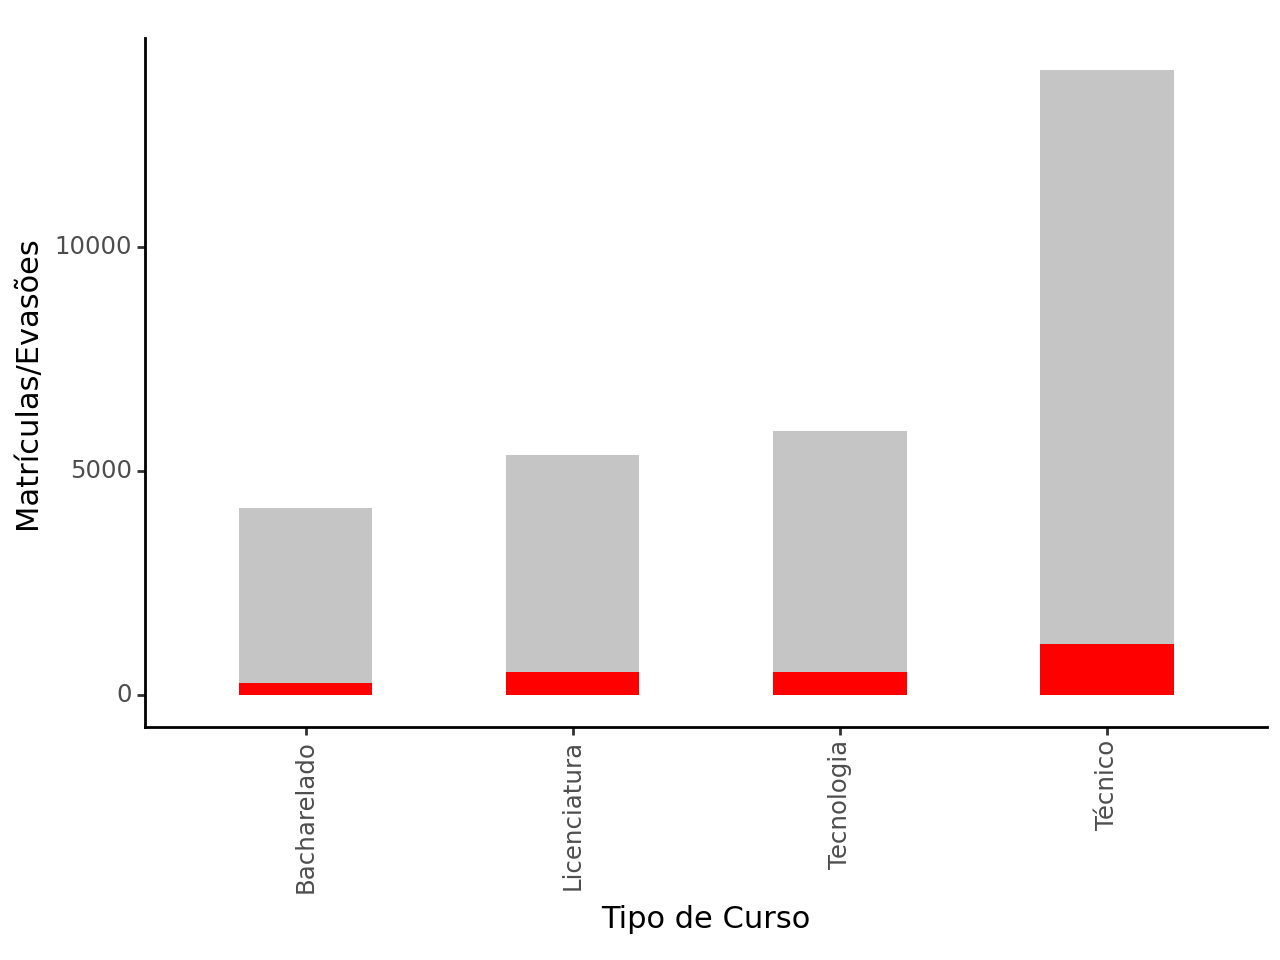
\includegraphics[width=8.9cm]{figs/figura-2.png}
    \centering
    Figura 2. Gráfico do tipo histograma representando o total de matrículas por tipo de curso, e a sobreposição contendo o número de evasões (em vermelho).
\end{figure}

\begin{figure}[h]
    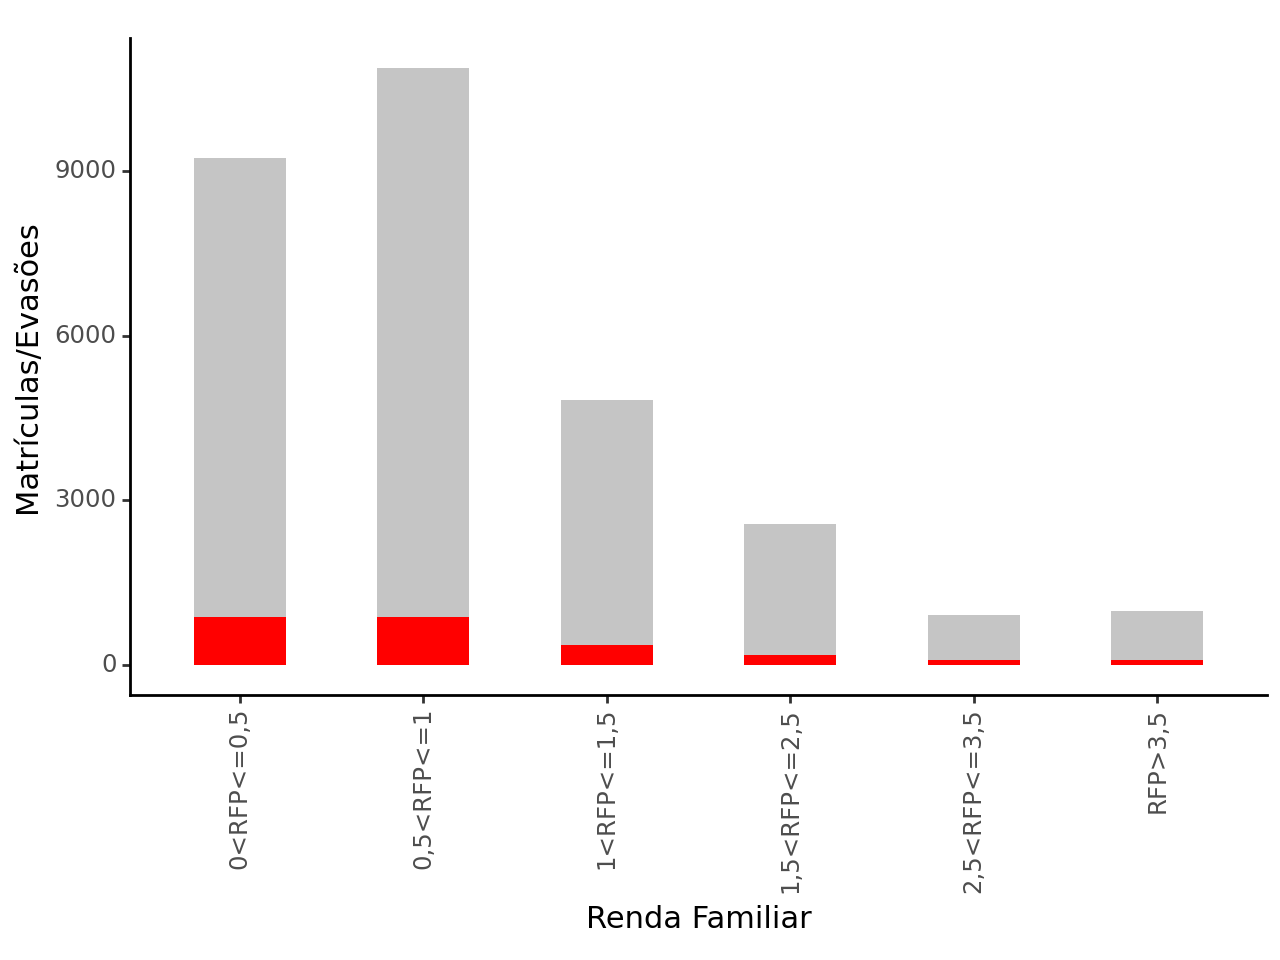
\includegraphics[width=8.9cm]{figs/figura-3.png}
    \centering
    Figura 3. Gráfico do tipo histograma representando o total de matrículas por categoria de renda familiar, e a sobreposição contendo o número de evasões (em vermelho).
\end{figure}

\begin{figure}[h]
    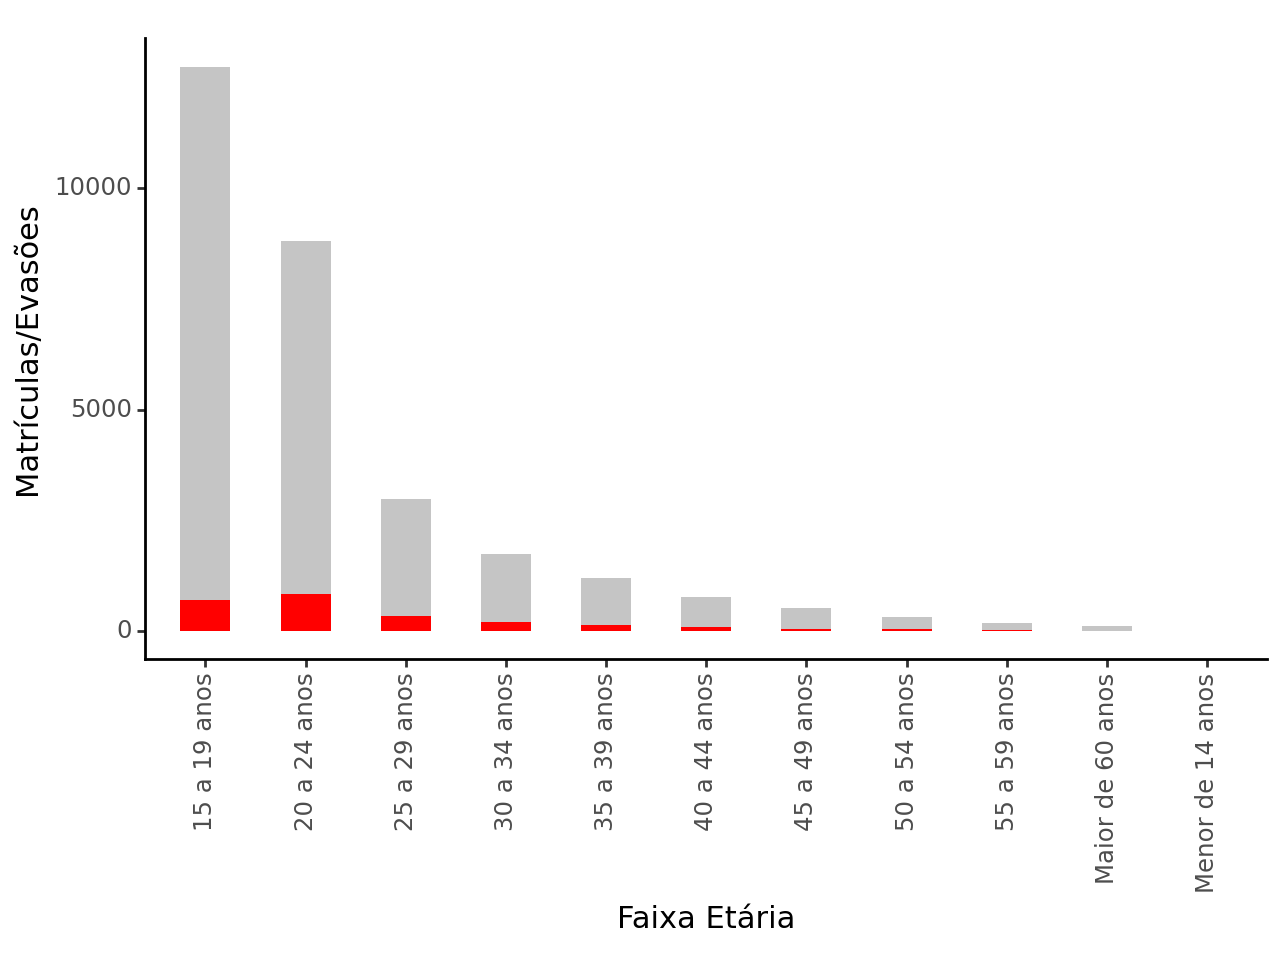
\includegraphics[width=8.9cm]{figs/figura-4.png}
    \centering
    Figura 4. Gráfico do tipo histograma representando o total de matrículas por faixa etária, e a sobreposição contendo o número de evasões (em vermelho).
\end{figure}

Para construção da análise objeto deste trabalho, parte-se da elaboração de uma hipótese, definida como hipótese nula (h-nada ou H\textsubscript{0}).\par
A hipótese nula (H\textsubscript{0}) definida para este estudo a partir do conjunto de dados a ser analisado fica definida como: "a evasão dos estudantes matriculados no IFSP não é influenciada pela renda familiar do estudante". E a hipótese alternativa (H\textsubscript{1}) sendo o seu inverso: "a evasão dos estudantes matriculados no IFSP é influenciada pela renda familiar do estudante".\par
Para elaboração deste estudo de hipótese será necessária a análise da correlação das distribuições de valores de duas variáveis categóricas: "Renda Familiar" e "Evasão".\par
A verificação e validação da hipótese nula (H\textsubscript{0}) será abordada de duas formas, primeiramente será analisado os resultados da distribuição de \raisebox{2pt}{$\chi$}\textsuperscript{2} (distribuição qui-quadrado ou chi-squared distribution) para verificar se as variáveis analisadas são independentes (independência ou independence in contingency tables), confirmando a hipótese nula (H\textsubscript{0}).\par
O cálculo realizado pelo teste da distribuição qui-quadrado segue a fórmula:\par

\[ \chi_{v}^{2} = \sum_{k=1}^{n} \frac{(O_k - E_k)^2}{E_k} \]

Onde:

\begin{itemize}
    \item n é a quantidade de categorias na variável
    \item O é o valor observado de uma determinada classe
    \item E é o valor esperado desta classe
    \item v é o grau de liberdade, número de determinações independentes menos o número de parâmetros estatísticos a serem avaliados
\end{itemize}

Desta forma, a distribuição qui-quadrado é a distribuição desta estatística sobre repetidas amostragens retiradas do modelo nulo. Analisando a fórmula deduzimos que quanto maior a diferença entre as frequências observadas e esperadas, maior será a estatística do teste.\par
Para utilização do teste qui-quadrado, alguns pressupostos são necessários, como: os dados serem aleatórios e representativos da população; as frequências esperadas serem maiores ou iguais a 1 e cada observação pertencer somente a uma categoria. A definição do resultado final, que confirma ou anula, a hipótese nula é realizada a partir da comparação do valor estatístico do teste com o valor crítico, que é obtido a partir da Tabela de Distribuição de Qui-Quadrado que apresenta os valores críticos de qui-quadrado para diferentes níveis de significância e graus de liberdade.\par
Na variável "Renda Familiar" possuímos um grau de liberdade de valor 5 (Ver Tabela 1 para descrição dos valores da variável). O grau de liberdade pode ser obtido através da fórmula:
\[ gl = R - 1 \]
Onde R representa o número de categorias da variável observada.\par
Considerando as seis categorias existentes (Tabela 1) na variável "Renda Familiar", temos o grau de liberdade de valor 5.

\begin{center}
    \begin{tabular}{ |c|c| } 
        \hline
        \textbf{RFP} & \textbf{Renda por pessoa} \\
        \hline
        0<RFP<=0,5 & entre R\$ 0,00 e R\$ 500,00 \\
        \hline
        0,5<RFP<=1 & entre R\$ 500,00 e R\$ 1.000,00 \\
        \hline
        1<RFP<=1,5 & entre R\$ 1.000,00 e R\$ 1.500,00 \\
        \hline
        1,5<RFP<=2,5 & entre R\$ 1.500,00 e R\$ 2.500,00 \\
        \hline
        2,5<RFP<=3,5 & entre R\$ 2.500,00 e R\$ 3.500,00 \\ 
        \hline
        RFP>3,5 & acima de R\$ 3.500,00 \\
        \hline
    \end{tabular} \\
    Tabela 1: Categorias de Renda Familiar
\end{center}

A renda familiar per capita ou renda familiar por pessoa (RFP) \cite{franz2024}, é um valor utilizado pelo governo para comprovação de participação dos programas do governo federal. É calculado com base na soma da renda de todos os moradores de uma residência, dividida pelo número total de pessoas que vivem sob manutenção desta renda total.\par
O segundo passo de avaliação dos resultados consiste na análise do intervalo de confiança e do valor-p a partir da reamostragem com reposição (técnica Bootstrap) no conjunto de dados de matrículas cujos estudantes evadiram. O objetivo desta análise seria, uma vez que a hipótese nula fosse anulada, as classes de renda poderiam determinar uma tendência de resultado maior para evasão?\par
A partir de então uma nova hipótese nula (H\textsubscript{0}) seria avaliada: "não há diferença significativa nas proporções de evasão entre estudantes de diferentes categorias de renda familiar". E a hipótese alternativa (H\textsubscript{1}): "há uma diferença significativa nas proporções de evasão entre estudantes de diferentes categorias de renda familiar". Onde a estatística de interesse seria a diferença nas proporções de evasão entre duas categorias de renda familiar.\par
Por termos variáveis categóricas, para a simulação deste teste, foi necessário a atribuição de valores às faixas de renda familiar. Neste caso, aplicando um valor médio para cada faixa de renda, como apresentado na Tabela 2.

\begin{center}
    \begin{tabular}{ |c|c| } 
        \hline
        \textbf{RFP} & \textbf{Valor Mapeado} \\
        \hline
        0<RFP<=0,5 & 0,25 \\
        \hline
        0,5<RFP<=1 & 0,75 \\
        \hline
        1<RFP<=1,5 & 1,25 \\
        \hline
        1,5<RFP<=2,5 & 2,0 \\
        \hline
        2,5<RFP<=3,5 & 3,0 \\
        \hline
        RFP>3,5 & 4,0 \\
        \hline
    \end{tabular} \\
    Tabela 2: Valor médio mapeado para as Categorias de Renda Familiar
\end{center}

Para calcular a variação entre o valor zero, as categorias de renda foram aglutinadas em duas possibilidades: "baixa renda" para as categorias de renda cujo valor médio ficasse abaixo do salário mínimo à época de referência dos dados, no caso R\$ 1.045,00. E as demais rendas nomeadas como "alta renda".

\section{Resultados}
Para não nos limitarmos pela apreciação intuitiva que ao olhar os dados levam-nos a algumas conclusões, aplicamos algumas abordagens para o teste de hipóteses, que de seguida podemos ver os resultados para cada um dos casos.\par

Teste Qui-Quadrada\par
Considerando que há 6 categorias de valores na variável "renda familiar", temos 5 graus de liberdade, e para um nível de significância de 5\% encontramos o valor de qui-quadrado crítico de 11,07.\par
Os testes calculados entre as variáveis "Renda Familiar" e "Evasão", retornam um valor de qui-quadrado de 19.83 e valor-p de 0. Desta forma conseguimos descartar a hipótese nula, uma vez que o valor de qui-quadrado é superior ao valor crítico e o valor-p está dentro do nível de significância. Evidenciando que há uma dependência entre estas variáveis.\par

Além da variável renda familiar, fizemos o cálculo de qui-quadrado com outras variáveis presentes na base de dados, como "Faixa Etária", "Tipo de Curso", "Sexo" e "Cor/Raça" (Tabela 3). Nos testes apenas a variável "Cor/Raça" apresentou um resultado de qui-quadrado inferior ao valor crítico e valor-p fora do nível de significância.\par

\begin{center}
    \begin{tabular}{ |c|c|c| } 
        \hline
        \textbf{Variável} & \textbf{Qui-quadrado} & \textbf{Valor-p} \\
        \hline
        Faixa Etária & 381.25 & 0.00 \\
        \hline
        Tipo de Curso & 52.07 & 0.00 \\
        \hline
        Sexo & 28.61 & 0.00 \\
        \hline
        Renda Familiar & 19.83 & 0.00 \\
        \hline
        Cor/Raça & 7.77 & 0.17 \\
        \hline
    \end{tabular} \\
    Tabela 3. Resultados dos testes de qui-quadrado com as variáveis da base de dados.
\end{center}

A Figura 5 nos permite visualizar um percentual por classe de renda entre os alunos evadidos e não evadidos.\par

\begin{figure}[h]
    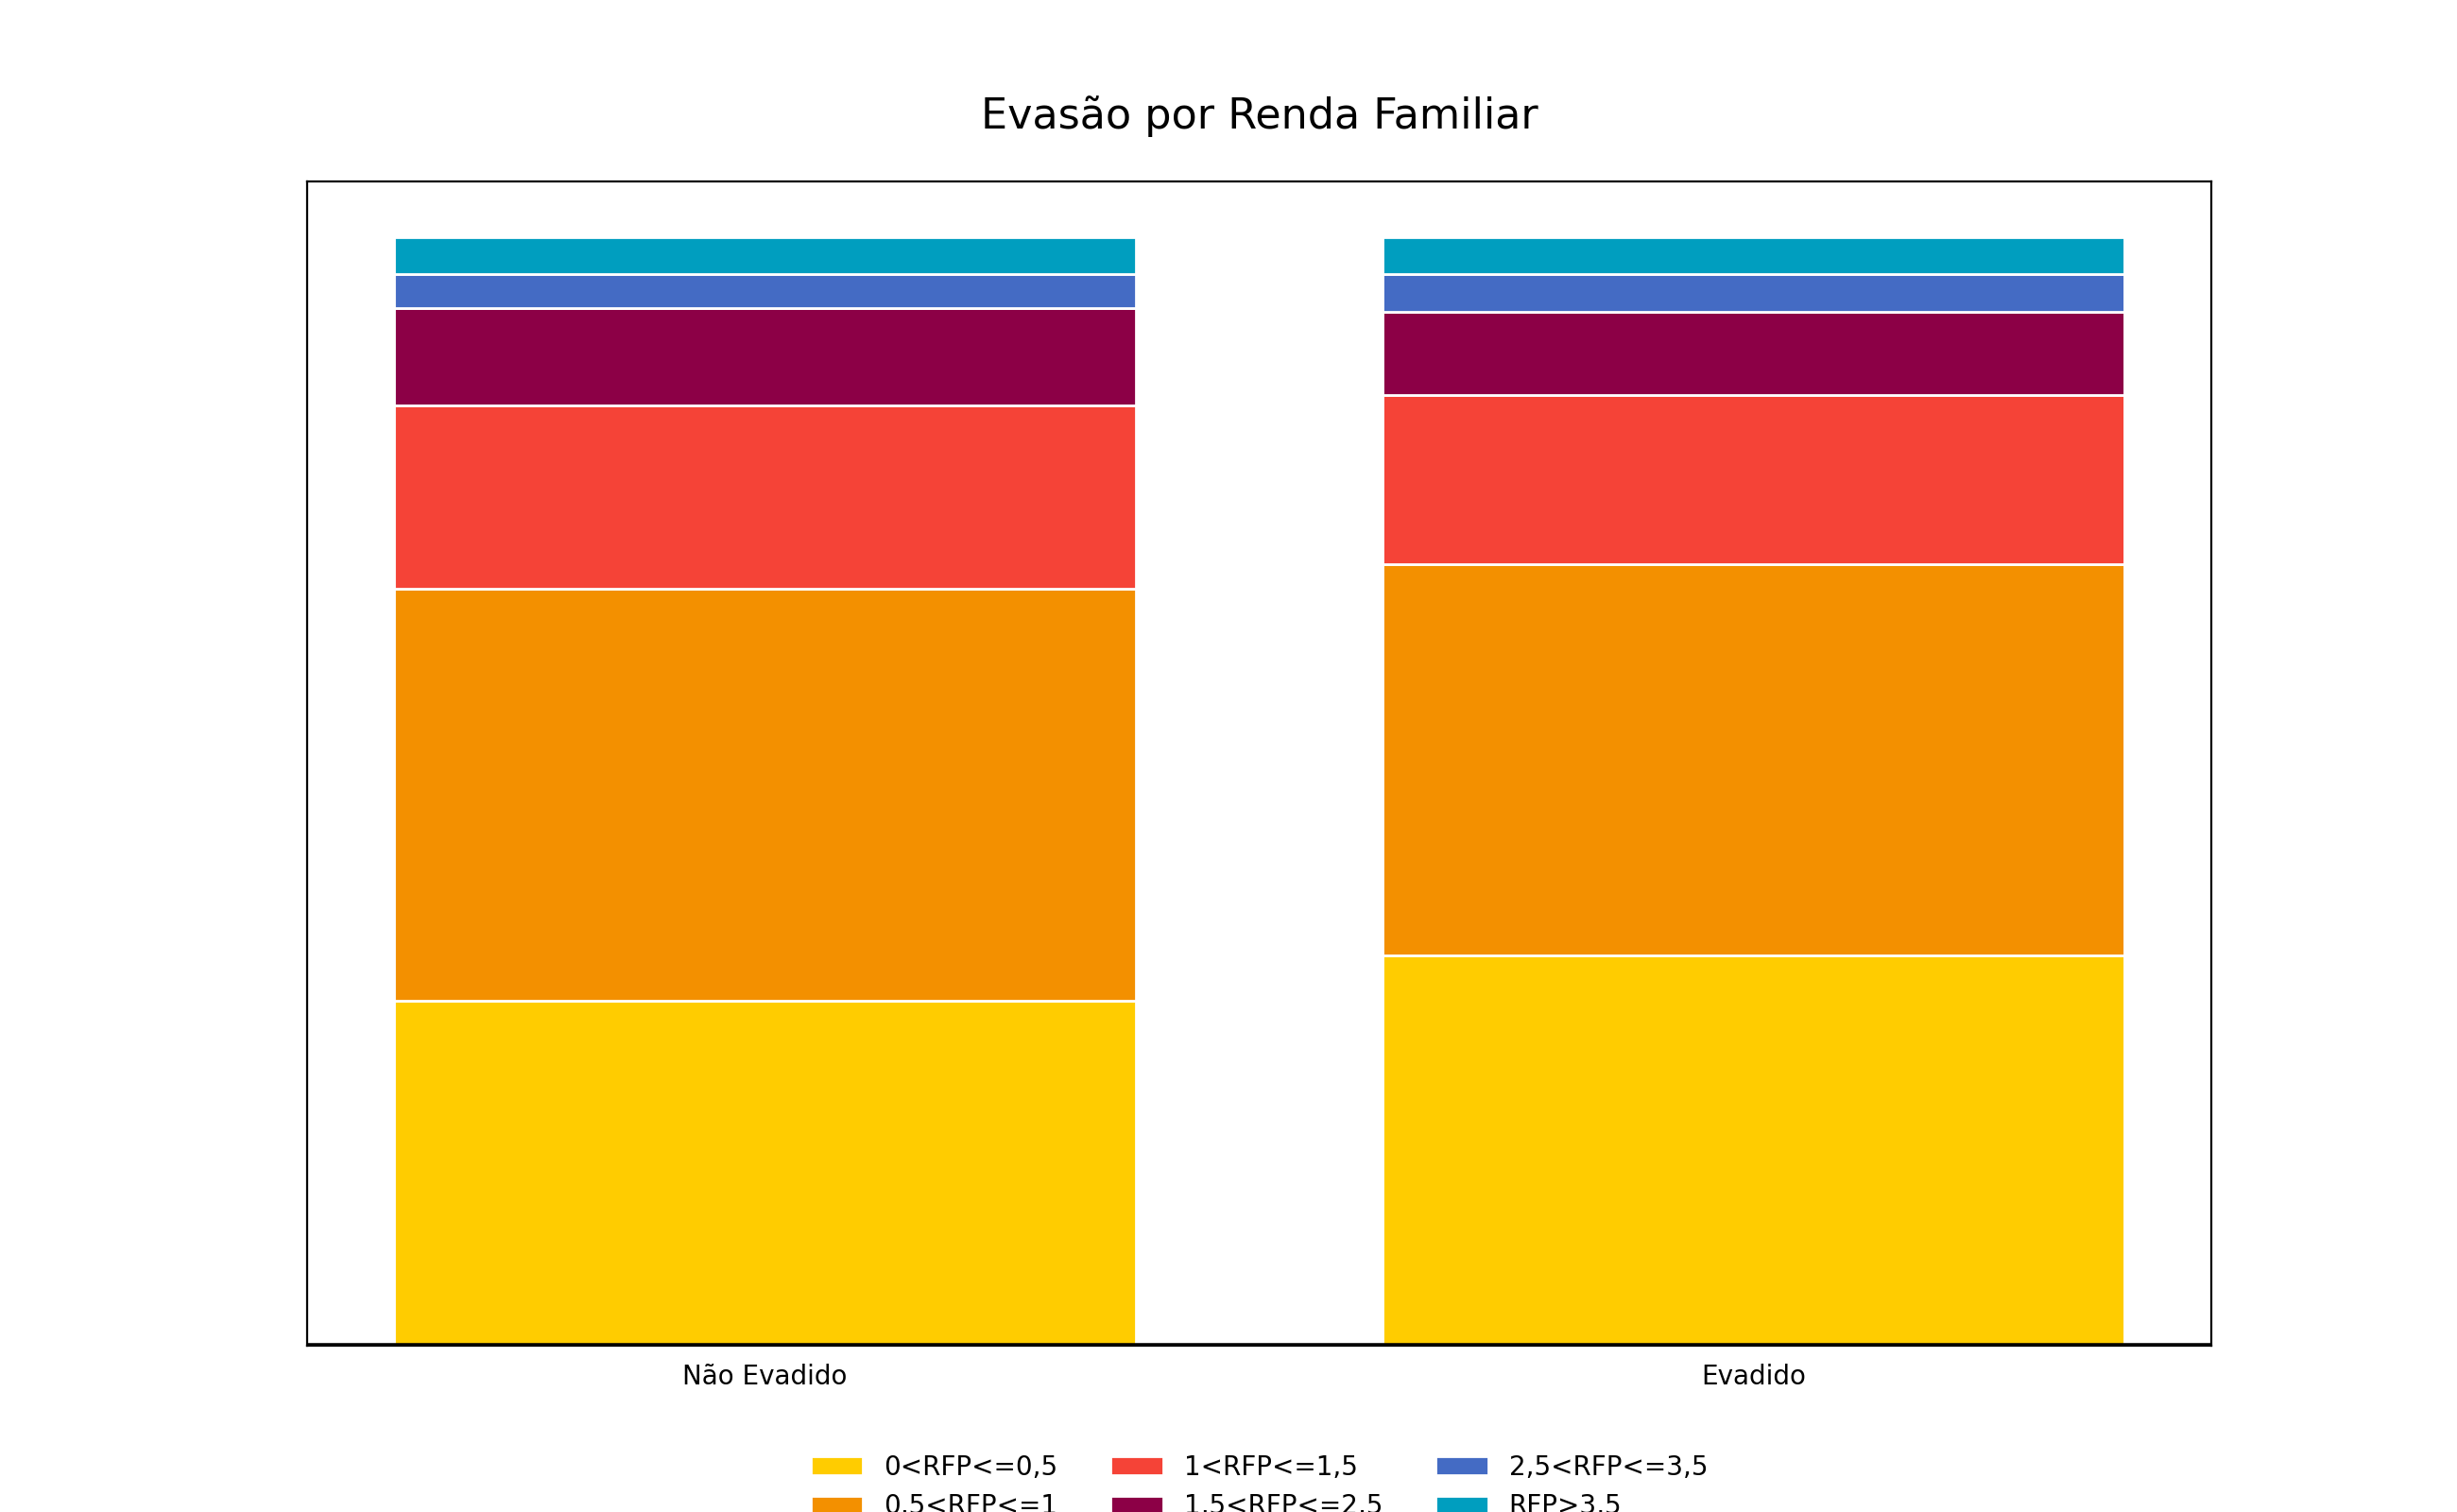
\includegraphics[width=8.9cm]{figs/figura-6.png}
    \centering
    Figura 5. Percentuais por classe de renda que contribuem para estudantes evadidos e não evadidos.
\end{figure}

Análise do Intervalo de Confiança e do Valor-p\par

Aplicando a técnica Bootstrap (reamostragem com reposição) no conjunto de dados de evadidos tanto de baixa renda, quanto os de alta renda, com um número de iterações 10.000, calculando a diferença entre a média dos casos de baixa renda e os casos de alta renda para cada amostra, e com tais diferenças gerar a sua distribuição para a nossa análise, suprindo a limitante de não ter os dados da população toda e ainda assim com base aos resultados obtidos podermos realizar a inferência das estatísticas dessas amostras à população.\par

\begin{figure}[h]
    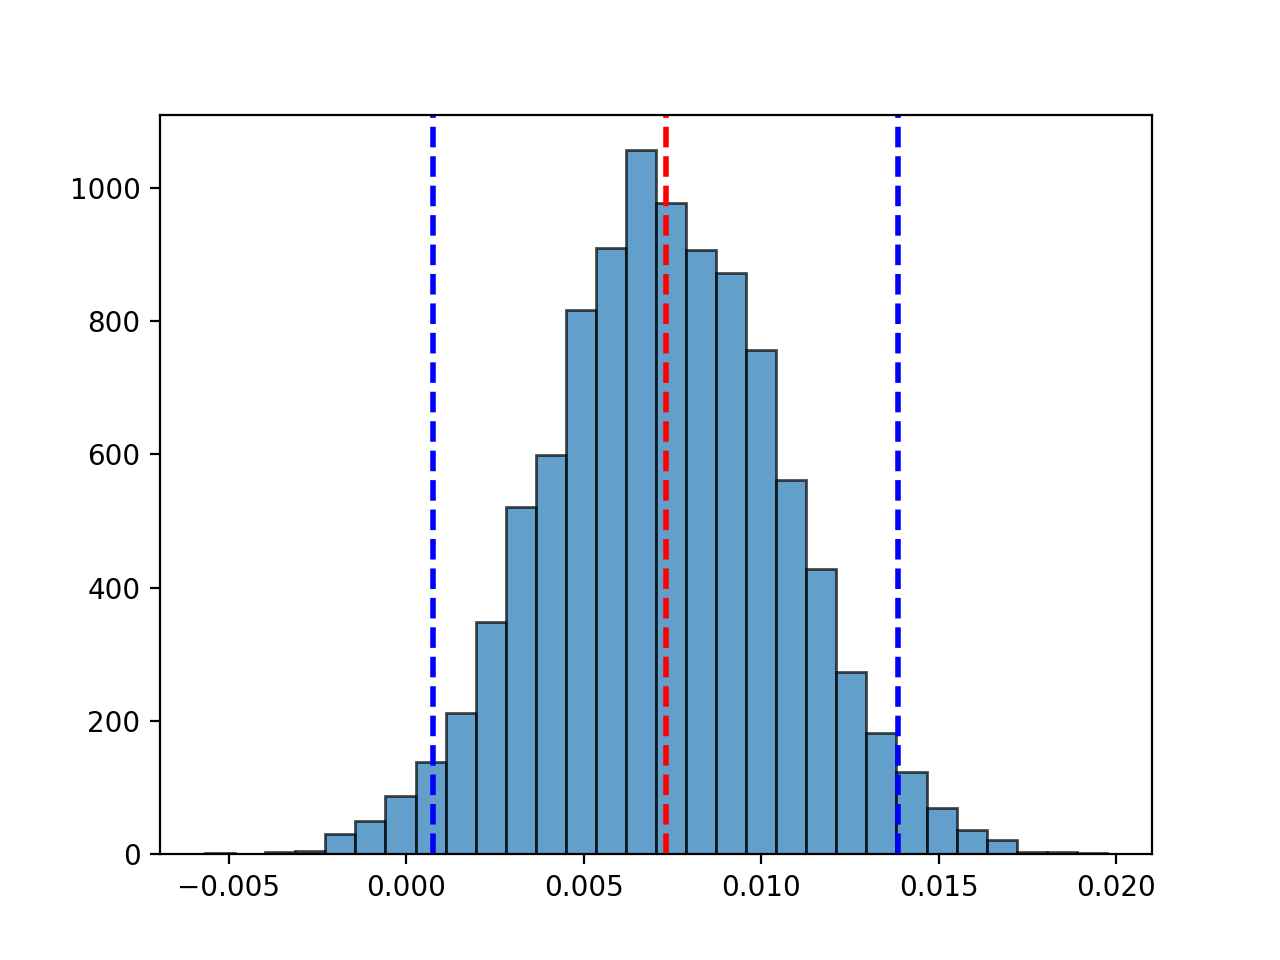
\includegraphics[width=8.9cm]{figs/figura-5.png}
    \centering
    Figura 6. Distribuição das diferenças de taxas de evasão.
\end{figure}

Diferença Observada (entre as Médias de Casos de Baixa Renda e as Médias de Casos de Alta Renda): 0.007326193492215388\par
Intervalo de Confiança(95%): [0.0007651976944975696, 0.01384664580579898]\par
valor-p: 0.4888

\section{Discussão}
Termos usado mais de uma abordagem para a análise da influência que tem a renda familiar de cada estudante na chance de converter-se em um caso de evasão, levou-nos a inicialmente a temer alguma discórdia nos resultados, mas o que percebemos no final é a complementaridade entre essas abordagens e os resultados que obtivemos dela, como por exemplo conseguimos perceber, tanto através do Qui-Quadrado, quanto pelo Intervalo de Confiança, ambos apontam para a rejeição da nossa Hipótese nula (H\textsubscript{0}), ou seja, confirmam que a ideia inicialmente intuitiva de que a renda familiar influencia no nível de invasão de estudantes, ao passo que o valor-p sugere uma maior especificidade de que este fator “pode” até influenciar, mas não há significância estatística suficiente para rejeitamos a hipótese H\textsubscript{0}, para dizer que o nível de evasão possa na verdade ser influenciado por vários fatores distintos e combinados. 

\section{Conclusões}
Pelas análises e testes de hipóteses elaborados por este trabalho, pode-se observar que a hipótese nula (H\textsubscript{0}) foi descartada, evidenciada pelo teste qui-quadrado, comprovando que a variável "Renda Familiar" influencia a evasão de estudantes. Porém não conseguimos determinar que uma determinada categoria de renda seja determinante sobre as demais categorias. Podemos observar esta percepção pela variação dos percentuais de contribuição das classes de renda em cada uma das situações de evasão, como demonstrada na figura 5.\par
Além disso, a renda familiar não é a única variável a contribuir para a evasão. Podemos notar que outras variáveis em conjunto, como faixa de idade e tipo de curso contribuem para evasão dos estudantes.\par
Desta forma não conseguimos com os estudos atuais e as variáveis presentes na base de dados, elaborar um modelo que possa determinar quais fatores contribuem em maior significância para este problema. Há a necessidade de mais informações e estudos envolvendo dados com um histórico maior e possivelmente correlacionar as matrículas anteriores com taxas de evasão mais recentes.


\selectlanguage{brazil}
\begin{thebibliography}{1}

\bibitem{oliveira2021} F. L. de Oliveira e L. Nóbrega, “Evasão escolar: um problema que se perpetua na educação brasileira”, vol. 21, nº 19, 25 de maio de 2021. Acesso em: 25 de junho de 2024. [Online]. Disponível em: https://educacaopublica.cecierj.edu.br/artigos/21/19/evasao-escolar-um-problema-que-se-perpetua-na-educacao-brasileira

\bibitem{silveira2021} F. R. da Silveira, A  evasão  de  estudantes  no  IFSP:  uma  contribuição  ao  conhecimento  das  dificuldades  na  identificação  de  seus determinantes. São Paulo: EDIFSP, 2021. Acesso em: 25 de junho de 2024. [Online]. Disponível em: https://editora.ifsp.edu.br/edifsp/catalog/view/11/11/45

\bibitem{pnp2024} Ministério da Educação, “PNP - Plataforma Nilo Peçanha”. Acesso em: 13 de junho de 2024. [Online]. Disponível em: https://www.gov.br/mec/pt-br/pnp

\bibitem{ismay2024} C. Ismay e A. Y. Kim, “Statistical Inference via Data Science - A ModernDive into R and the Tidyverse”, A ModernDive into R and the Tidyverse. Acesso em: 14 de junho de 2024. [Online]. Disponível em: https://moderndive.com.

\bibitem{pnpdados2024} Ministério da Educação, “PNP - Dados Abertos - MEC”, PNP - Dados Abertos - MEC. Acesso em: 14 de junho de 2024. [Online]. Disponível em: https://dadosabertos.mec.gov.br/pnp

\bibitem{microdados2021} Ministério da Educação, “2020 - Microdados Matrículas - Portal de Dados Abertos do Ministério da Educação”, Portal de Dados Abertos do Ministério da Educação. Acesso em: 14 de junho de 2024. [Online]. Disponível em: https://dadosabertos.mec.gov.br/pnp/item/134-2020-microdados-matriculas.

\bibitem{python2024} Python Software Foundation, “Welcome to Python.org”. Acesso em: 26 de junho de 2024. [Online]. Disponível em: https://www.python.org/

\bibitem{pandas2024} NumFOCUS, Inc., “pandas - Python Data Analysis Library”. Acesso em: 26 de junho de 2024. [Online]. Disponível em: https://pandas.pydata.org/

\bibitem{numpy2024} NumPy team, “NumPy”. Acesso em: 26 de junho de 2024. [Online]. Disponível em: https://numpy.org.

\bibitem{plotnine20204} H. Kibirige, “plotnine 0.13.6 - A Grammar of Graphics for Python”. Acesso em: 26 de junho de 2024. [Online]. Disponível em: https://plotnine.org

\bibitem{matplot2024} The Matplotlib development team, “Matplotlib: Visualization with Python”. Acesso em: 26 de junho de 2024. [Online]. Disponível em: https://matplotlib.org.

\bibitem{seaborn2024} M. Waskom, “Seaborn: statistical data visualization”. Acesso em: 26 de junho de 2024. [Online]. Disponível em: https://seaborn.pydata.org.

\bibitem{scipy2024} SciPy, “SciPy”. Acesso em: 26 de junho de 2024. [Online]. Disponível em: https://scipy.org.

\bibitem{statsmodel2024} J. Perktold, Seabold, e J. Taylor, “Statsmodels - statistical models, hypothesis tests, and data exploration”. Acesso em: 26 de junho de 2024. [Online]. Disponível em: https://www.statsmodels.org/stable/index.html.

\bibitem{franz2024} S. Frantz, “O que é renda per capita familiar”. [Online]. Disponível em: https://www.serasa.com.br/blog/renda-per-capita-familiar/.

\end{thebibliography}

\end{document}
